\documentclass[tikz]{standalone}
\usepackage{pgfplots}
\pgfplotsset{compat=1.15}
\usepackage{mathrsfs}
\usetikzlibrary{arrows,calc}
\usepackage{tkz-euclide}

\pagestyle{empty}

\definecolor{AngleClr}{rgb}{0,0.39215686274509803,0}
\definecolor{ShapeClr}{rgb}{0.6,0.2,0}

\begin{document}

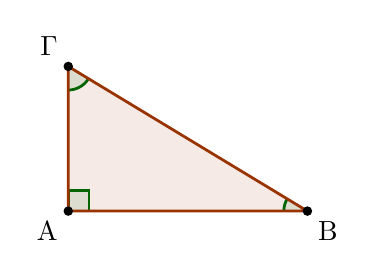
\begin{tikzpicture}[scale=.75]
\tkzSetUpLine[line width=1pt,color=black]
\tkzSetUpPoint[fill=black]

\tkzDefPoints{0/0/B,4.05/0/C}

\tkzDefPoint(90:2.45){A}

\tkzFillPolygon[fill=ShapeClr,fill opacity=0.1](A,B,C)

\tkzFillAngles[fill=AngleClr,size=.4,fill opacity=0.1](B,A,C A,C,B)
\tkzMarkAngles[line width=1pt,size=.4,color=AngleClr](B,A,C A,C,B)

\tkzMarkRightAngle[line width=1pt, size=.35,color=AngleClr,fill=AngleClr,fill opacity=0.1](A,B,C)

\tkzDrawPolygon[color=ShapeClr](A,B,C)

\tkzDrawPoints[size=3](A,B,C)
\tkzLabelPoint[above left](A){$\mathrm{\Gamma}$}
\tkzLabelPoint[below left](B){$\mathrm{A}$}
\tkzLabelPoint[below right](C){$\mathrm{B}$}

\end{tikzpicture}

\end{document}
